\documentclass{beamer}

\usepackage[english]{babel}

\usepackage[latin1]{inputenc}

\usepackage{times}
\usepackage{hyperref}
\usepackage{listings}
\usepackage{comment}
\usepackage{booktabs} % for toprule
\usepackage{tikz}
\usetikzlibrary{positioning}

\lstset{frame=none, showstringspaces=false, basicstyle=\footnotesize,
  xleftmargin=-8mm,language=Haskell}

\newcommand{\colAwidth}{0.1\textwidth}
\newcommand{\colBwidth}{0.8\textwidth}

\title[GOOL]{Multi-lingual code generation in Drasil}

\author{\underline{Jacques Carette}, Spencer Smith, Dan Szymczak and
Steven Palmer}

\institute[McMaster University]{McMaster University}

\date[July 2017]{WG 2.11, July 2017 Meeting}

\beamertemplatenavigationsymbolsempty 

\begin{document}

%I will present some ongoing work that seeks to generate all the artifacts
%involved in software (obviously code, but also specification documents, design
%documents, tests, user manual, Makefiles, etc). In the context of software
%which requires (re)certification, all of these artifacts are involved -- and
%they normally contain a huge amount of duplicate information. Our approach is
%to do very aggressive knowledge encapsulation, followed by relatively
%straightforward generation passes. For domains (such as scientific computation)
%where there is well-established theory, our preliminary experiments shows that
%this works quite well. Note that we do NOT expect this to work so well in
%domains without well-established theory.

\begin{frame}
\titlepage
\end{frame}

\begin{frame}

\includegraphics{generate_all_the_things.jpg}
\end{frame}

\begin{frame}

\includegraphics[width=\textwidth]{no_silver_bullet.jpg}
\end{frame}

% Drasil
%%% - generate all the things
%%% - no silver bullet
%%% - context
%%% * example: doc (D) + code (S) (GlassBR)
%%% - ontologies (D)
%%%   * go through well-formatted Data.Drasil.Concepts.*, Data.Drasil.SI_Units
%%%       (D - if you could make sure these are as clean as possible?)
%%%   - typeclasses of Language.Drasil (D) [esp. as this has evolved a lot recently]
%%%   * Example.Drasil.DocumentLanguage.

\begin{frame}
\frametitle{Context}
{\Large software \onslide<2->{(re)}certification}
\vspace*{.2cm}
\begin{itemize}
\item<3->All software artifacts as \textcolor{green}{evidence}:
\begin{itemize}
\item \textcolor{blue}{requirements, software specification, software design, code, 
  tests, ``theory manual'', user manual, \ldots}
\end{itemize}
\vspace*{.5cm}
\item<4->Massive amounts of \textcolor{red}{knowledge duplication}
\begin{itemize}
  \item Implies that either
  \begin{itemize}
    \item non-code artifacts do not get maintained well enough, OR
    \item are felt to be an expensive nuisance
  \end{itemize}
  \item duplication harms traceability
\end{itemize}
\end{itemize}
\vfill
\end{frame}

\begin{frame}
\frametitle{Examples}
\begin{itemize}
\item {\color{blue}GlassBR}: Computer whether a given plate of glass will resist a blast force.
\item GamePhysics: ``Chipmunk'' game physics engine.
\item SSP: Computation of mixed-soil slop stability.
\item SWHS: Solar Water Heating System (w/ phase change material).
\item NoPCM: Solar Water Heating System without PCM.
\item Tiny: convective and effective heat transfer coefficients.
\end{itemize}
\end{frame}

\begin{frame}[t]
\frametitle{Ontologies}
{\large \onslide<1->{\only<1>{\color{blue}}Data.Drasil} 
\onslide<2,3->{- \only<2>{\color{blue}}Language Concepts}
\onslide<3->{- \only<3->{\color{blue}}Document Language}}

\only<1>{
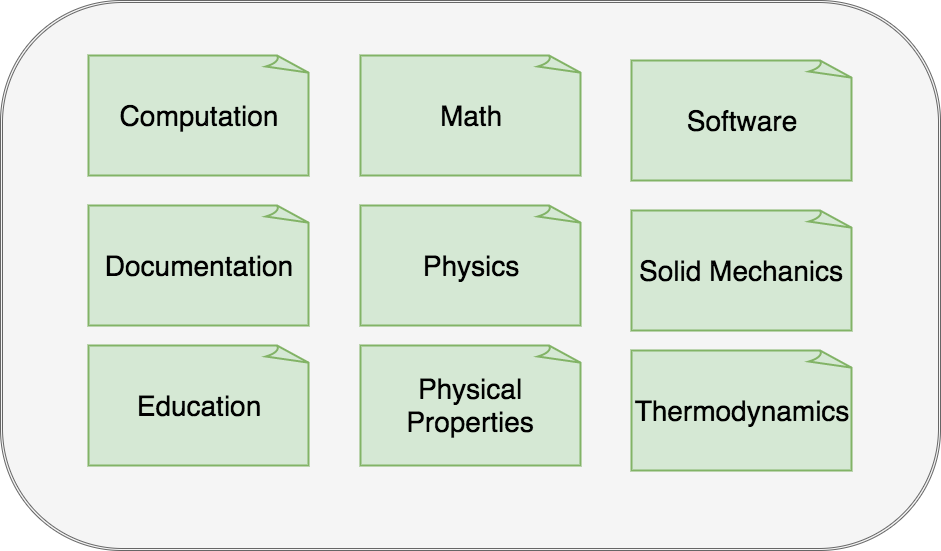
\includegraphics[scale=0.33]{Data_Drasil.png}
}
\only<2>{
\center{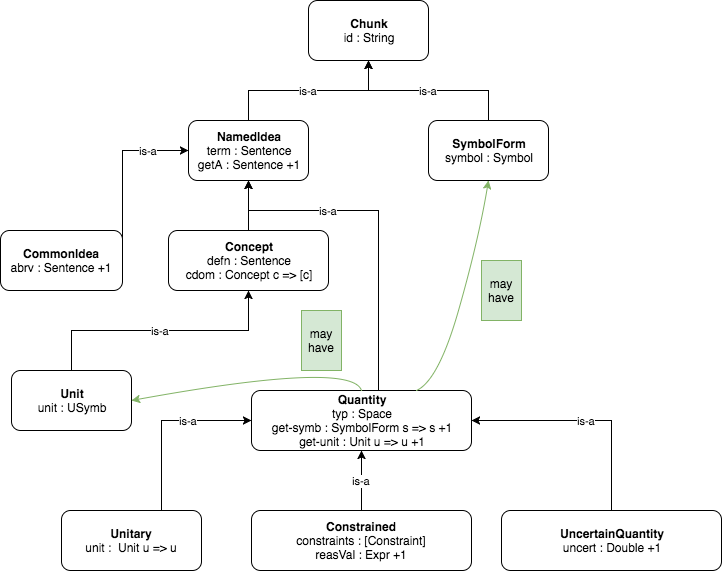
\includegraphics[scale=0.33]{class_hierarchy.png}}
}
\only<3>{
\vspace{2cm}
\emph{\Large{Show the details already!}}
}
\end{frame}

% Gool
% - origins (J)
% - design
%   - meta-language abstracting details (J)
%     - all required features of all languages (S?)
%        ex: public/private
%     - 7 language renderers (as virtual dispatch table - in Haskell!) (S)
%     - pretty-printer to make things look nice
%     - lots of smart constructors to make it look PL-like (give example) (S)
% 
% Choices
% - implementation choices, design choices, "aspects" (J)
% - examples of
%   - implementation choices (S)
%   - design choices (S) 

\begin{frame}

\includegraphics[width=0.48\textwidth]{generate_all_the_things.jpg}

\includegraphics[width=0.48\textwidth]{no_silver_bullet.jpg}
\end{frame}

\end{document}
